\documentclass{beamer}

\usetheme{Madrid}
\usecolortheme{default}
\usepackage{amsmath, amssymb}
\usepackage{graphicx}
\usepackage{algorithm}
\usepackage{algpseudocode}

% Define custom colors for emphasis
\definecolor{highlight}{RGB}{70,130,180}

\title{Achieving Optimal Blackjack Play Through Double Q-Learning}
\subtitle{COMP3106 Final Project}
\author{Qayam Damji, Shri Vaibhav Mahesh Kumar, Daniel Tam}
\institute{Carleton University}
\date{\today}

\begin{document}

\begin{frame}
    \titlepage
\end{frame}

\begin{frame}{Outline}
    \tableofcontents[hideallsubsections]
\end{frame}

\section{Introduction}

\begin{frame}{Background and Motivation}
    \begin{block}{Why Blackjack?}
        \begin{itemize}
            \item Perfect blend of skill and probability
            \item Well-defined rules with complex decision spaces
            \item Real-world application potential
            \item Ideal for testing AI adaptation capabilities
        \end{itemize}
    \end{block}
    
    \begin{block}{Research Goals}
        \begin{itemize}
            \item Develop optimal playing strategies using RL
            \item Test effectiveness of Double Q-Learning
            \item Compare performance against traditional strategies
            \item Integrate card counting for enhanced decision-making
        \end{itemize}
    \end{block}
\end{frame}

\begin{frame}{Related Prior Work}
    \begin{block}{Q-Learning Evolution}
        \begin{itemize}
            \item \textbf{Original Q-Learning (Watkins)}
                \begin{itemize}
                    \item Value function approximation
                    \item State-action pair evaluation
                    \item Temporal difference learning
                \end{itemize}
            \item \textbf{Double Q-Learning (van Hasselt)}
                \begin{itemize}
                    \item Addresses maximization bias
                    \item Dual estimator approach
                    \item Improved stability in stochastic environments
                \end{itemize}
        \end{itemize}
    \end{block}
    
    \begin{block}{Industry Applications}
        \begin{itemize}
            \item FAIR's poker AI breakthrough (2017)
            \item Professional player defeat milestone
            \item Reinforcement learning in imperfect information games
        \end{itemize}
    \end{block}
\end{frame}

\section{Blackjack Fundamentals}

\begin{frame}{Basic Game Rules}
    \begin{columns}
        \column{0.5\textwidth}
        \textbf{Card Values}
        \begin{itemize}
            \item 2-10: Face value
            \item Jack, Queen, King: 10
            \item Ace: 1 or 11 (flexible)
        \end{itemize}
        
        \textbf{Objective}
        \begin{itemize}
            \item Beat dealer's hand
            \item Get closest to 21
            \item Don't exceed 21 (bust)
        \end{itemize}
        
        \column{0.5\textwidth}
        \textbf{Player Actions}
        \begin{itemize}
            \item Hit: Request another card
            \item Stand: Keep current hand
            \item Split: Divide matching pairs
            \item Double Down: Double bet, one card
        \end{itemize}
    \end{columns}
\end{frame}

\begin{frame}{Dealer Rules and Game Flow}
    \begin{block}{Dealer Constraints}
        \begin{itemize}
            \item Must hit on 16 or below
            \item Must stand on hard 17 or above
            \item Some casinos require hit on soft 17
            \item No splitting or doubling down
        \end{itemize}
    \end{block}
    
    \begin{block}{Game Resolution}
        \begin{itemize}
            \item Player bust: Immediate loss
            \item Dealer bust: All standing players win
            \item Higher hand wins (if no busts)
            \item Equal hands: Push (tie)
            \item Natural blackjack pays 3:2
        \end{itemize}
    \end{block}
\end{frame}

\begin{frame}{Card Counting Fundamentals}
    \begin{block}{Hi-Lo System}
        \begin{itemize}
            \item \textbf{Low cards (2-6):} +1
            \item \textbf{Mid cards (7-9):} 0
            \item \textbf{High cards (10-A):} -1
        \end{itemize}
    \end{block}
    
    \begin{block}{Running Count vs True Count}
        \begin{itemize}
            \item Running Count = Sum of card values seen
            \item True Count = Running Count ÷ Decks Remaining
            \item Positive count: Advantage to player
            \item Negative count: Advantage to dealer
        \end{itemize}
    \end{block}
\end{frame}

\section{Methodology}

\begin{frame}{State Space Design}
    \textbf{State Space Components:}
    \[(player\_value, has\_usable\_ace, dealer\_upcard, count\_bucket, is\_pair, pair\_value)\]
    
    \begin{itemize}
        \item \textbf{player\_value} \(\in\) [4,21]
        \item \textbf{has\_usable\_ace} \(\in\) {0,1}
        \item \textbf{dealer\_upcard} \(\in\) [1,10]
        \item \textbf{count\_bucket} \(\in\) {-1,0,1}
        \item \textbf{is\_pair} \(\in\) {0,1}
        \item \textbf{pair\_value} \(\in\) [0,10]
    \end{itemize}
\end{frame}

\begin{frame}{Action Space and Constraints}
    \textbf{Action Space:} \(A = \{0 \text{ (Stand)}, 1 \text{ (Hit)}, 2 \text{ (Split)}\}\)
    
    \begin{block}{Action Constraints}
        \begin{itemize}
            \item \textbf{Stand (0):}
                \begin{itemize}
                    \item Always available
                    \item Ends player's turn
                \end{itemize}
            \item \textbf{Hit (1):}
                \begin{itemize}
                    \item Available if not busted
                    \item Draws one card
                \end{itemize}
            \item \textbf{Split (2):}
                \begin{itemize}
                    \item Requires matching pair
                    \item Maximum 3 splits
                    \item Each hand gets new card
                \end{itemize}
        \end{itemize}
    \end{block}
\end{frame}

\begin{frame}{Q-Learning Implementation}
    \begin{block}{Core Update Equation}
        \[Q(s,a)\leftarrow Q(s,a)+\alpha[r(s)+\gamma\max_{a^\prime}Q(s^\prime,a^\prime)-Q(s,a)]\]
        Where:
        \begin{itemize}
            \item $\alpha$: Learning rate
            \item $\gamma$: Discount factor
            \item $r(s)$: Immediate reward
            \item $s'$: Next state
        \end{itemize}
    \end{block}
    
    \begin{block}{Dynamic Learning Rate}
        \[\alpha(s,a) = \max(\alpha_0 \cdot \delta^{N(s,a)}, \alpha_{\min})\]
        \begin{itemize}
            \item $N(s,a)$: Visit count
            \item $\delta$: Decay rate
            \item $\alpha_0$: Initial learning rate
            \item $\alpha_{\min}$: Minimum learning rate
        \end{itemize}
    \end{block}
\end{frame}

\begin{frame}{Double Q-Learning Implementation}
    \begin{block}{Dual Q-Tables}
        \begin{itemize}
            \item Maintains two Q-value estimators ($Q_1$, $Q_2$)
            \item Reduces overestimation bias
            \item Randomly updates one table per step
        \end{itemize}
    \end{block}
    
    \begin{block}{Update Function}
        \[Q_1(s,a) \leftarrow Q_1(s,a) + \alpha[R + \gamma Q_2(s',\arg\max_{a'} Q_1(s',a')) - Q_1(s,a)]\]
        Key Features:
        \begin{itemize}
            \item Action selection from $Q_1$
            \item Value estimation from $Q_2$
            \item Decorrelated maximum value estimation
        \end{itemize}
    \end{block}
\end{frame}

\begin{frame}{Reward Structure}
    \begin{equation*}
        R(p,d) = \begin{cases}
        -1.2b & \text{if } p > 21 \text{ (bust)} \\
        1.1b & \text{if } d > 21 \text{ (dealer bust)} \\
        1.5b & \text{if } p = 21 \text{ (natural)} \\
        1.1b & \text{if } p > d \text{ and } p \geq 20 \\
        b & \text{if } p > d \\
        -b & \text{if } p < d \\
        0 & \text{if } p = d
        \end{cases}
    \end{equation*}
    Where:
    \begin{itemize}
        \item $p$: Player's hand value
        \item $d$: Dealer's hand value
        \item $b$: Base reward unit
    \end{itemize}
\end{frame}

\begin{frame}{Epsilon-Greedy Exploration}
    \begin{block}{Action Selection Probability}
        \begin{equation*}
            P(a|s) = \begin{cases}
            1-\epsilon + \frac{\epsilon}{|A|} & \text{if } a = \arg\max_{a'} Q(s,a') \\
            \frac{\epsilon}{|A|} & \text{otherwise}
            \end{cases}
        \end{equation*}
    \end{block}
    
    \begin{block}{Adaptive Exploration Rate}
        \begin{equation*}
            \epsilon = \max(\epsilon_{\min}, \epsilon \cdot \begin{cases}
            \delta_\epsilon \cdot 1.1 & \text{if improving} \\
            \delta_\epsilon & \text{otherwise}
            \end{cases})
        \end{equation*}
    \end{block}
\end{frame}

\begin{frame}{Training Results}
    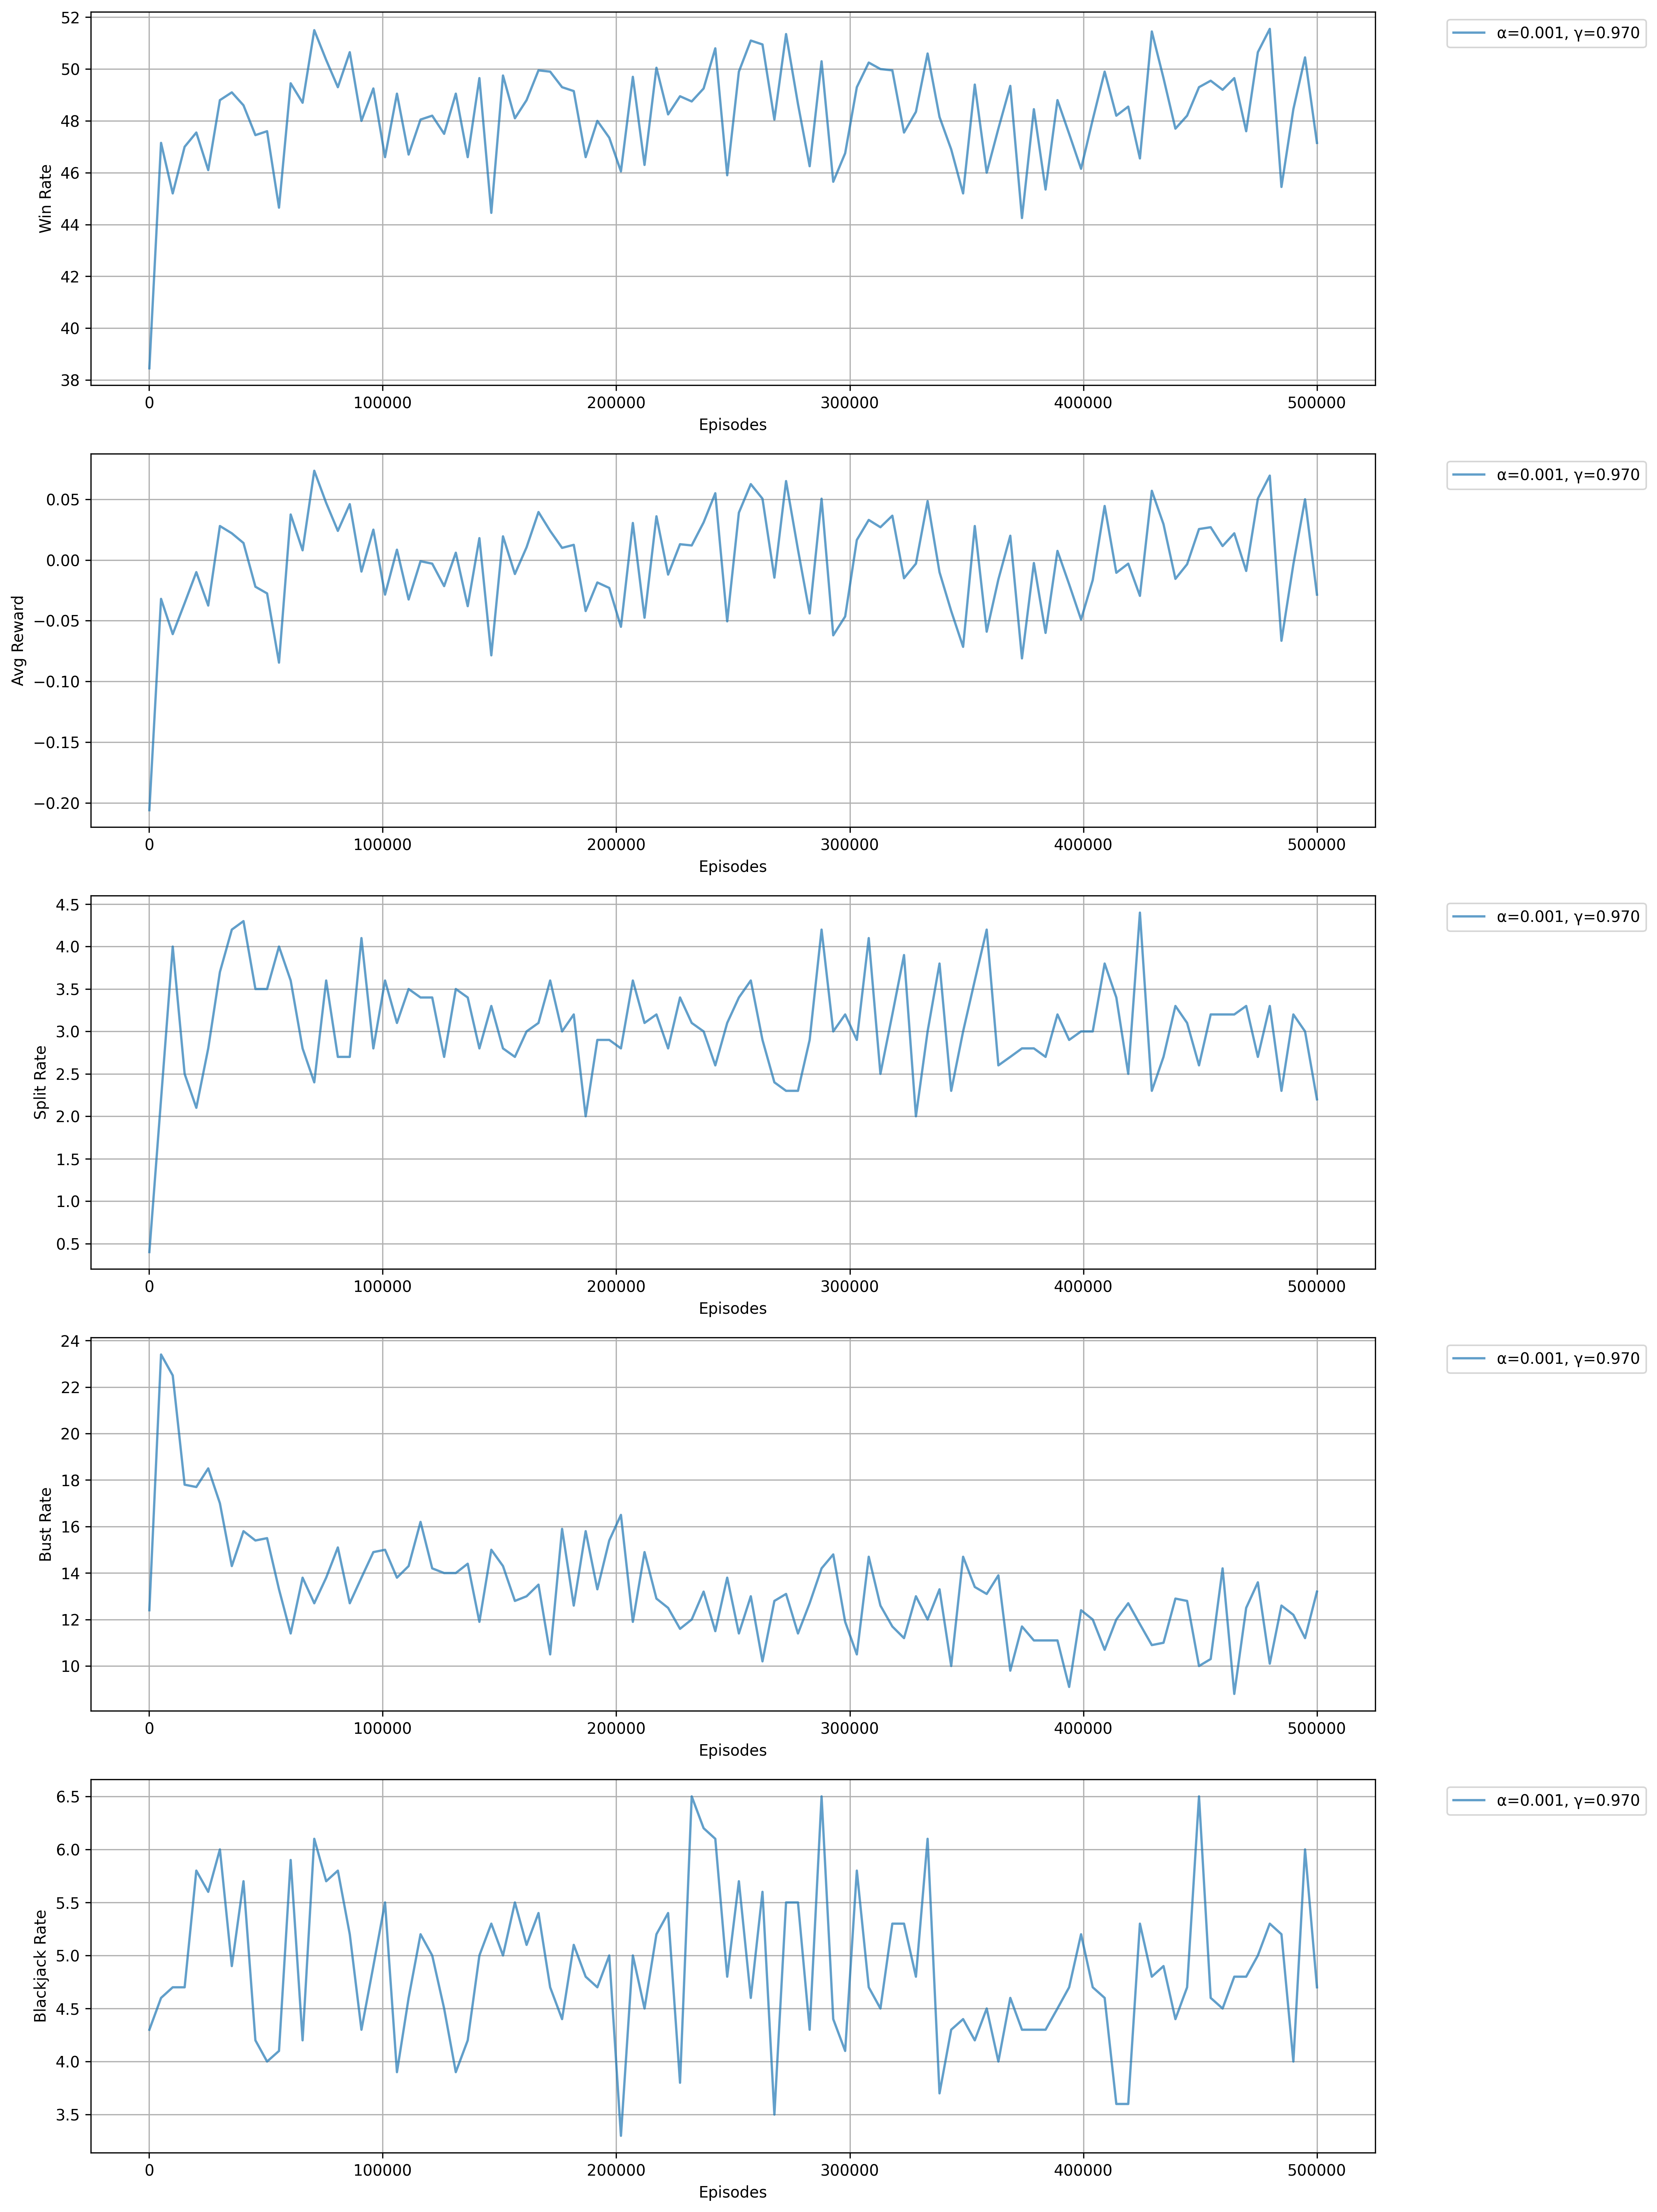
\includegraphics[width=\textwidth]{./images/learning_curves_summary.png}
    
    \begin{block}{Final Performance Metrics}
        \begin{itemize}
            \item Win rate: 48.05\% (approaches theoretical maximum)
            \item Average reward: -0.003 (minimal house edge impact)
            \item Split rate: 3.05\% (conservative splitting)
            \item Blackjack rate: 5.3\% (matches theoretical probability)
            \item Bust rate: 10.95\% (significant improvement from >20\%)
        \end{itemize}
    \end{block}
\end{frame}

\begin{frame}{Strategy Analysis}
    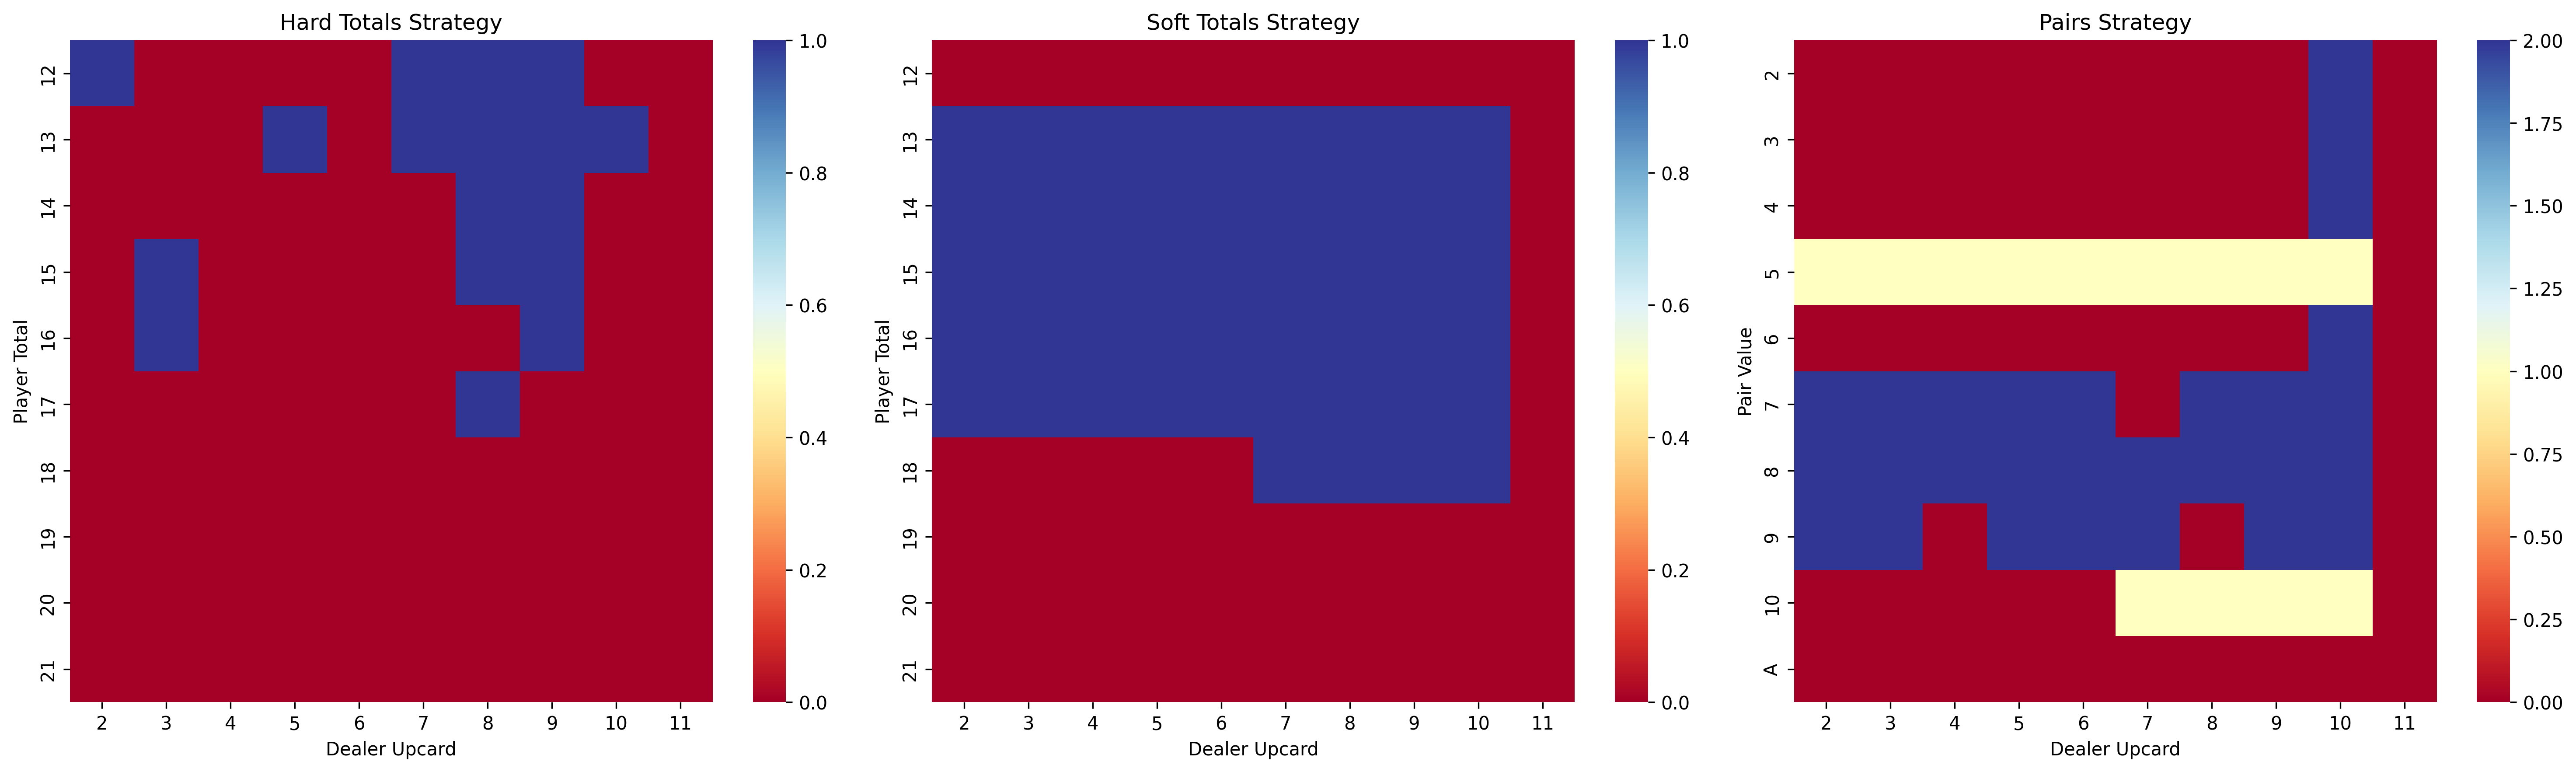
\includegraphics[width=\textwidth]{./images/agent_strategy.png}
    
    \begin{columns}
        \column{0.5\textwidth}
        \textbf{Hard Totals}
        \begin{itemize}
            \item Stand on 17+
            \item Hit on 16- vs high cards
            \item Conservative vs dealer 2-6
        \end{itemize}
        
        \column{0.5\textwidth}
        \textbf{Soft Totals}
        \begin{itemize}
            \item Hit below soft 18
            \item Stand on soft 19+
            \item Strategic soft 18 play
        \end{itemize}
    \end{columns}
\end{frame}

\section{Discussion}

\begin{frame}{Limitations}
    \begin{block}{Performance Ceiling}
        \begin{itemize}
            \item Win rate plateau at 48-50\%
            \item Inherent house edge challenge
            \item Approaches theoretical maximum
        \end{itemize}
    \end{block}
    
    \begin{block}{Strategic Gaps}
        \begin{itemize}
            \item Suboptimal split rate (3.05\%)
            \item Room for reward function refinement
            \item Casino simulation fidelity limitations
        \end{itemize}
    \end{block}
\end{frame}

\begin{frame}{Future Directions}
    \begin{block}{Technical Improvements}
        \begin{itemize}
            \item Enhanced split strategy training
            \item More sophisticated reward shaping
            \item Deeper card counting integration
        \end{itemize}
    \end{block}
    
    \begin{block}{Real-World Applications}
        \begin{itemize}
            \item Dealer rule variations
            \item Multi-deck adaptability
            \item Real-time decision support
            \item Training tool development
        \end{itemize}
    \end{block}
\end{frame}

\end{document}